\documentclass{article}

\usepackage[margin=1in]{geometry}
\usepackage{amsmath}
\usepackage{amssymb}
\usepackage{mathtools}

\begin{document}

\title{M 476 - Homework 5}
\author{Nathan Stouffer}

\maketitle
\newpage

\section*{Problem 1}
Consider the two subsets
$X := \{ (x,y) \in \mathbb{R}^2 \mid xy = 0 \}$
and
$Z := \{ (w,z) \in \mathbb{C}^2 \mid wz = 0 \}$.
\subsection*{Part A}
Problem: Show that both $X$ and $Z$ are path-connected. \\\\
Solution: We first consider $X$. We will build a continuous map from an arbitrary point in $X$ to the origin of $\mathbb{R}^2$.
For an element $(x,y) \in X$, we know, by the definition of $X$, that either $x$ or $y$ must be 0.
Without loss of generality, take $x = 0$.
Then, we must map an arbitrary $y$ to 0 on the real number line. This is done by
$f: [0,1] \to \mathbb{R}$,
specifically,
$t \mapsto ty$.
The map $f$ must be continuous by obs (prod).
Furthermore,
$0 \mapsto 0$ and $1 \mapsto y$.
Therefore, the set $X$ must be path-connected. \\\\
We now show, through a similar argument, that $Z$ is path-connected. We will build a continuous map from an arbitrary point in $Z$ to the origin of the complex plane.
For an element $(w,z) \in Z$, we know, by the definition of $Z$, that either $w$ or $z$ must be the complex number 0.
Without loss of generality, take $w = 0$.
Then, we must map an arbitrary $z$ to the origin of the complex plane. This is done by
$f: [0,1] \to \mathbb{C}$,
specifically,
$t \mapsto tz$.
The map $f$ must be continuous by obs (prod).
Furthermore,
$0 \mapsto 0$ and $1 \mapsto z$.
Thus the set $Z$ is path-connected.
\subsection*{Part B}
Problem: For each finite cardinality $r$, identify the subsets
$Cut_r(X) \subset X$ and $Cut_r(Z) \subset Z$. \\\\
We begin with the set $X$. \\
In the case $r = 0$: $Cut_0(X) = \emptyset$ \\
In the case $r = 1$: $Cut_1(X) = \emptyset$ \\
In the case $r = 2$: $Cut_2(X) = \{ (x,y) \in \mathbb{R}^2 \mid (x,y) \neq (0,0) \} $ \\
In the case $r = 3$: $Cut_3(X) = \emptyset$ \\
In the case $r = 4$: $Cut_4(X) = \{ (0,0) \}$ \\
In the case $r > 5$: Since no two sets of cut points in $X$ will intersect and all elements of $X$ are accounted for in the above cases, any $r > 5$ will produce an empty set. \\\\
We now move to the set $Z$. \\
In the case $r = 0$: $Cut_0(Z) = \emptyset$ \\
In the case $r = 1$: $Cut_1(Z) = \{ (w,z) \in \mathbb{C}^2 \mid (w,z) \neq (0,0) \} $ \\
In the case $r = 2$: $Cut_2(Z) = \{ (0,0) \} $ \\
In the case $r > 3$: Since no two sets of cut points in $Z$ will intersect and all elements of $Z$ are accounted for in the above cases, any $r > 3$ will produce an empty set.

\newpage

\section*{Problem 2}
Problem: Let $n > 0$. Consider the subset
$$U_n := \{ U \in GL_n(\mathbb{R}) \mid U \text{ is upper triangular} \} \subset GL_n(\mathbb{R}) \subset Mat_{n \times n}(\mathbb{R}) \cong \mathbb{R}^{n^2}$$
For each $n > 0$, identify the cardinality of $| \pi_o (U_n(\mathbb{R})) |$. \\\\
Solution: We begin with an arbitrary $n \times n$ matrix $A$ and note that $A$ is really just $n \times n$ slots for real numbers. Thus the slots must be filled with $\mathbb{R}^{n^2}$.
Now, an element $U^ \prime \in U_n$ has constraints on the input.
The matrix $U^\prime$ must be upper triangular and invertible. For such a $U^\prime$, the values in the diagonal of $U^\prime$ must all be nonzero. Thus, the slots of $U^\prime$ must be filled with
$ \{ 0 \}^{\times {n \choose 2}} \times (\mathbb{R} \setminus O)^n \times \mathbb{R}^{\times {n \choose 2}}$. \\\\
We now apply the proposition that, given two sets $X$ and $Y$,
$\pi_o (X \times Y)$ is bijective with $\pi_o (X) \times \pi_o (Y)$.
We also note that bijective sets must have equal cardinalities.
Using this proposition, since $|\pi_o (\{ 0 \})| = 1$, it must be true that $|\pi_o (\{ 0 \} ^ {\times {n \choose 2}})| = 1$.
Likewise, since $|\pi_o (\{ \mathbb{R} \})| = 1$, it must be true that $|\pi_o (\{ \mathbb{R} \} ^ {\times {n \choose 2}})| = 1$.
The proposition can be used again to show that
$ \pi_o (U_n(\mathbb{R})) $
is bijective with
$ \pi_o (\mathbb{R} \setminus O)^n $.
Since the two sets are bijective, their cardinality must be equal. Thus,
$| \pi_o (U_n(\mathbb{R})) | = | \pi_o (\mathbb{R} \setminus O)^n | $. \\\\
We know that $ | \pi_o (\mathbb{R} \setminus O) | = 2$. Therefore, by the same proposition as before, $ | \pi_o (\mathbb{R} \setminus O)^n | = 2^n$.
Thus, for $n > 0$, $| \pi_o (U_n(\mathbb{R})) | = 2^n$.

\newpage

\section*{Problem 3}
Problem: For $n = 2$ and $n = 3$, prove that $P_n$ is finite and identify the cardinality $| P_n |$. \\\\
Solution: We begin by writing the definition of $P_n$.
$$ P_n := \{ (z_1, z_2, ... z_n) \in \mathbb{C}^{\times n} \mid z_1 = 0 \text{ and } z_2 = 1 \text{ and } dist(z_i, z_{i+1}) = 1 \text{ and } dist(z_n, z_1) = 1 \} \subset \mathbb{C}^{\times n} $$
We now examine the case $n = 2$. The set $P_2 = \{ (0, 1) \}$. Since $P_2$ has only one element, $P_2$ must be finite and $| P_2 | = 1$. \\\\
We now shift our focus to the case $n = 3$. The set $P_3 = \{ (0, 1, \dfrac{1}{2} + \dfrac{\sqrt{3}}{2}i), (0, 1, \dfrac{1}{2} - \dfrac{\sqrt{3}}{2}i) \}$
Since $P_3$ has two discrete elements, $P_3$ must be finite and $| P_3 | = 2$.

\newpage

\section*{Problem 4}
Problem: For each $n \geq 2$, identify the cardinality $| \pi_o (P_n) |$. \\\\
Solution: For cases $n = 2,3$, we have already shown in Problem 3 that
$| \pi_o (P_2) = 1 |$ and $| \pi_o (P_3) = 2 |$. \\\\
We now consider the case $n \geq 4$.
We will show that $| \pi_o (P_n) | = 1$ where $n \geq 4$ by induction.
Additionally, we will use the following statement: $| \pi_o (P_n) | = 1$ iff $P_n$ is path-connected. \\\\
Consider the base case of $n = 4$. The set $P_4$ is path-connected if we can build a continuous map from an arbitrary element in $P_4$ to the element $(0,1,0,1)$.
Take $(0,1,a_3,a_4)$ as an arbitrary element of $P_4$. While staying in $P_4$, we can rotate the position of $a_3$ to $0$. Given that we must stay in $P_4$, this will map $a_4$ to a point $a_4^\prime$, giving $(0,1,0,a_4^\prime)$.
We can now rotate the point $a_4^\prime$ to the point $1$, which gives $(0,1,0,1)$. Thus the base case is proved. \\\\
We now state the inductive assumption: Assume there exists $k \geq 4$ for which $P_{n = k}$ is path-connected. That is, assume, for an arbitrary $p = (0, 1, a_3, a_4, ... ,a_k) \in P_{n = k}$, there exists a continuous path in $P_{n = k}$ that maps $p$ to $(0,1,0,1, ... ,a^\prime _k) \in P_{n = k}$. \\\\
We will now show that $P_{n = k + 1}$ must also be path-connected. Take $q = (0,1,a_3, a_4, ... , a_k, a_{k+1})$ as an arbitrary element of $P_{n = k + 1}$. By inductive assumption, we know that $q$ maps to $q^\prime = (0,1,0,1,..., a^\prime _k, a^\prime _{k+1})$. \\\\
There are now two cases: either $k$ is odd or $k$ is even. \\\\
Case $k$ is odd: Since $k$ is odd, the $k-1$ point in $q^\prime$ must be $1$. Then, while staying in $P_{n = k + 1}$, we can then rotate $a^\prime _k$ to $0$, which gives
$(0,1,0,1,... ,0,a^{\prime \prime}_{k+1}) \in P_{n = k + 1}$.
Now, $a^{\prime \prime}_{k+1}$ can be rotated to be $1$, yielding $(0,1,0,1,...,0,1) \in P_{n = k + 1}$. Thus, in the case that $k$ is odd, $P_{n = k + 1}$ is path-connected. \\\\
Case $k$ is even: Since $k$ is even, the $k-1$ point in $q^\prime$ must be $0$. Then, while staying in $P_{n = k + 1}$, we can then rotate $a^\prime _k$ to $1$, which gives
$q^{\prime \prime} = (0,1,0,1,... ,1,a^{\prime \prime}_{k+1}) \in P_{n = k + 1}$.
Since $q^{\prime \prime} \in P_{k + 1}$, it must be the case that
$a^{\prime \prime} _{k + 1} = \dfrac{1}{2} + \dfrac{\sqrt{3}}{2}i$
or $a^{\prime \prime} _{k + 1} = \dfrac{1}{2} - \dfrac{\sqrt{3}}{2}i$. \\\\
We must now show that both cases of $q^{\prime \prime}$ are path connected. That is, we must show that there is a continuous map from 
$X = (0,1,0,1,... ,1,\dfrac{1}{2} + \dfrac{\sqrt{3}}{2}i) \in P_{k + 1} $ to
$Y = (0,1,0,1,... ,1,\dfrac{1}{2} - \dfrac{\sqrt{3}}{2}i) \in P_{k + 1} $
in $P_{k+1}$
This is done in the figure on the following page.
\newpage
\begin{figure}[h]
	\centering
	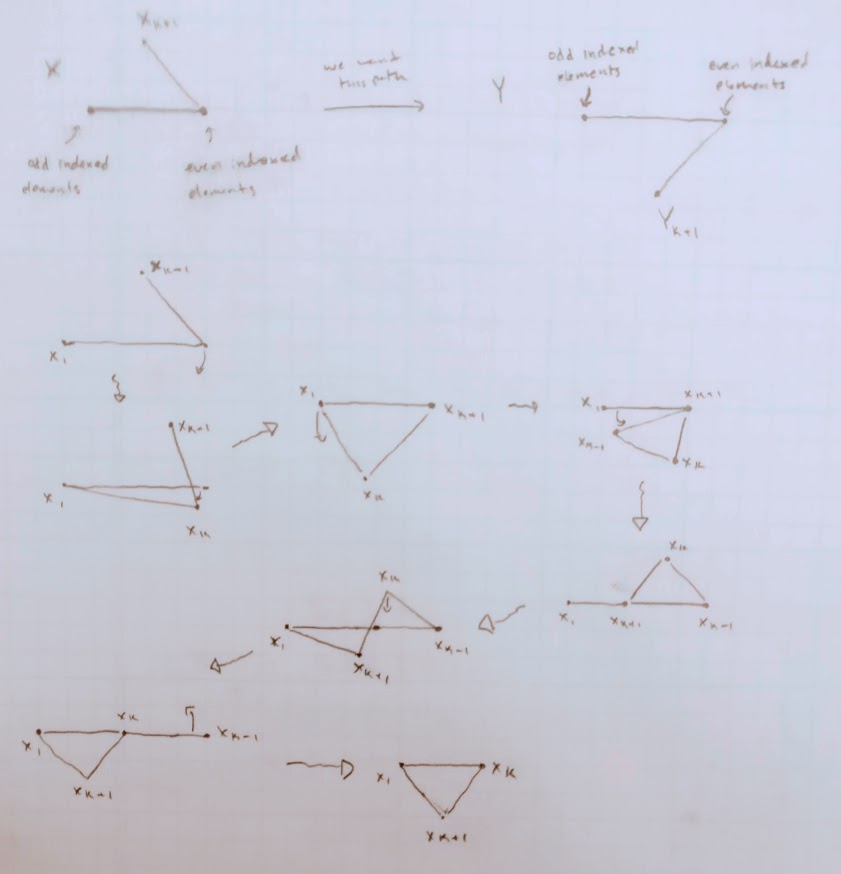
\includegraphics[width=5in]{path-connected.png}
\end{figure}
Thus, in the case that $k$ is odd, $P_{n = k + 1}$ is path-connected. \\\\
Since it has been inductively proven (in both the case that $k$ is odd and that $k$ is even) that $P_{n = k + 1}$ is path-connected. It must be true that $P_n$ is path-connected for $n \geq 4$. \\\\
Finally, since $P_n$ for $n \geq 4$ is path-connected, it must be true that $| \pi_o (P_n) | = 1$ for $n \geq 4$.

\newpage

\section*{Problem 5}
Problem: Identify a graph $X$ for which there is a homeomorphism $X \cong P_4$. \\\\
Solution: Consider the following set of elements of $P_4$:
$v = \{ (0,1,0,1), (0,1,0,-1), (0,1,2,1) \}$.
We now refer to Figure 1. 
\begin{figure}[h]
	\centering
	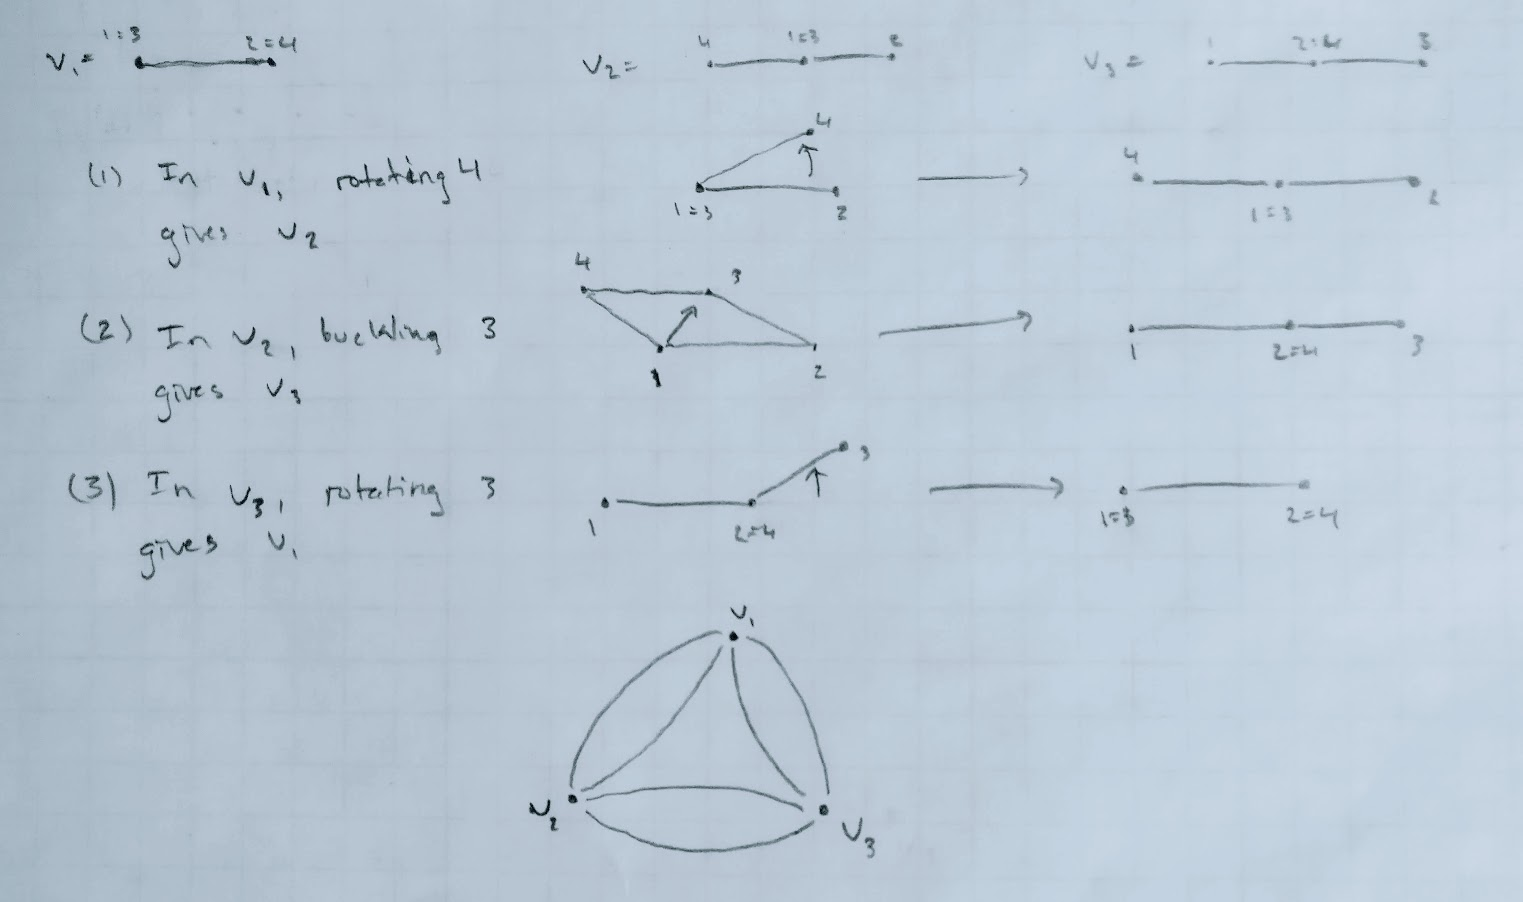
\includegraphics[width=5in]{P-sub-4-graph.png}
	\caption{Graph $X$ that is homeomorphic $P_4$}
\end{figure} \\
Consider the distinct operations (1), (2), and (3). Without loss of generality, take an operation $o$. The operation $o$ can be defined by an angle $\theta$.
Additionally, we could choose to define $o$ by the angle $- \theta$. Thus, for each operation, there are two directions to choose from.
The set of elements within those operations (excluding the set $v$) consist of edges in the graph $X$ since there is only one direction of travel and its opposite. \\\\
We now examine the elements in $v$. Such elements have four distinct choices for the direction of travel (two directions and their opposites). Thus the set $v$ is the set of vertices in the graph $X$. \\\\
For clarity, the graph $X$ is pictured in Figure 1.

\end{document}